\documentclass[../main.tex]{subfiles}

\graphicspath{{ima/clase19}{ima}}

% Aquí empieza el documento{{{
\begin{document}
\chapter{Funciones generadoras}%

\thispagestyle{fancy}

\textbf{Idea:} Usar los coeficientes de polinomios para responder
\dobledef{problemas}{o series} de conteo.

Si $a_n$ es la respuesta que buscamos, la encontramos como coeficiente de $x^n$
en una ``función formal'' es decir:
\[
	a_n =
	\underbrace
	{
		A(x)
	}_
	{
		\substack
		{
			\text{Función}\\
			\text{generadora}
		}
	}
	[x^n]
\]
\[
	A(x) = \sum_{k=0}^\infty a_kx^k
\]

Vuelto usando monedas de $1$ de $2$ y de $5$:
\[
	\underbrace
	{
		(x^0+x+x^2+x^3+\cdots)
	}_
	{
		\sum_{k=0}^\infty x^k
	}
	\underbrace
	{
		(x^0+x^2+x^4+x^6+x^8\cdots)
	}_
	{
		\sum_{k=0}^\infty x^{2k}
	}
	\underbrace
	{
		(x^0+x^5+x^{10}+\cdots)
	}_
	{
		\sum_{k=0}^\infty x^{5k}
	}
\]

Vuelto de 12:(Contribución por moneda)
\begin{table}[H]
	\centering
	\begin{tabular}{|c|c|c|}
		%$<++>$ & $<++>$ & $<++>$\\
		$1$ & $2$ & $5$\\
		\hline
		$12$ & $0$ & $0$\\
		$10$ & $2$ & $0$\\
		$8$ & $4$ & $0$\\
		$6$ & $6$ & $0$\\
		$4$ & $6$ & $0$\\
		$2$ & $10$ & $0$\\
		$0$ & $12$ & $0$\\
		\hline
		$7$ & $0$ & $5$\\
		$5$ & $2$ & $5$\\
		$3$ & $4$ & $5$\\
		$1$ & $6$ & $5$\\
		\hline
		$2$ & $0$ & $10$\\
		$0$ & $2$ & $10$\\
	\end{tabular}
\end{table}
\[
	(x^0+x+x^2+x^3+\cdots)
	(x^0+x^2+x^4+\cdots)=
\]
\[
	\underbrace
	{
		1+x^1+(x^2+x^2)+2x^3+3x^4+\cdots
	}_
	{
		\sum_{k=0}^\infty b_k x^k = B(x)
	}
\]
\[
	(b_k)_{k=0}^\infty \underset{1:1}{\longleftrightarrow}
	\underset{\sum_{k=0}^\infty b_kx^k}{B(x)}
\]

\section{Polinomios torre:}%
\label{sec:polinomios_torre_}

\begin{figure}[H]
	\centering
	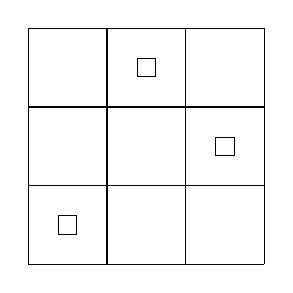
\begin{tikzpicture}[scale=1, transform shape]
		\draw[step=1] (0,0) grid ++(3,3);
		\node[rectangle, draw] at (0.5,0.5) {};
		\node[rectangle, draw] at (2.5,1.5) {};
		\node[rectangle, draw] at (1.5,2.5) {};
	\end{tikzpicture}
\end{figure}

(Las torres son indistinguibles entre sí)
(La tabla tiene solo una orientación)

¿Cuántas formas hay que poner distintos números de torres en el ``tablero''
sin que estas se ataquen entre sí?

Espacios para cada torre: (3 torres, 9 cuadrados)
\[
	\frac
	{
		\overbrace
		{
			9
		}^
		{
			\substack
			{
				\text{Para la}\\
				\text{primera}\\
				\text{torre}
			}
		}
		*
		\overbrace
		{
			4
		}^
		{
			\substack
			{
				\text{Para la}\\
				\text{segunda}\\
				\text{torre}
			}
		}
		*
		\overbrace
		{
			1
		}^
		{
			\substack
			{
				\text{Para la}\\
				\text{última}\\
				\text{torre}
			}
		}
	}
	{
		\underbrace
		{
			3!
		}_
		{
			\substack
			{
				\text{Porque son}\\
				\text{indistinguibles}
			}
		}
	}
	=6
\]
\[
	P_t(x)[x^k]: \substack
	{
		\text{\# de formas de poner $k$}\\
		\text{torres en el tablero $T$}\\
		\text{sin que se ataquen entre sí.}
	}
\]
\tikzset
{
	bloque/.pic=
	{
		\filldraw (0,0) rectangle ++(0.5/3,0.5/3);
	}
}

\[
	P_
	{
		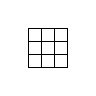
\begin{tikzpicture}[scale=1, transform shape]
			\draw[step={0.5/3}] (0,0) grid ++(0.5,0.5);
		\end{tikzpicture}
	}
	(x)
	=xP_
	{
		\begin{tikzpicture}[scale=1, transform shape]
			\draw[step={0.5/3}] (0,0) grid ++(0.5,0.5);
			\pic at (0,0) {bloque};
			%\filldraw (0,0) rectangle ++(0.5/3,0.5/3);
			\filldraw (0,0.5/3) rectangle ++(0.5/3,0.5/3);
			\filldraw (0.5/3,1/3) rectangle ++(0.5/3,0.5/3);
			\filldraw (1/3,1/3) rectangle ++(0.5/3,0.5/3);
		\end{tikzpicture}
	}(x)
	+P_
	{
		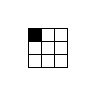
\begin{tikzpicture}[scale=1, transform shape]
			\draw[step={0.5/3}] (0,0) grid ++(0.5,0.5);
			\filldraw (0,1/3) rectangle ++(0.5/3,0.5/3);
		\end{tikzpicture}
	}
	(x)
\]
\[
	P_
	{
		\begin{tikzpicture}[scale=1, transform shape]
			\draw[step={0.5/3}] (0,0) grid ++(0.5,0.5);
			\pic at (0,0) {bloque};
			\pic at (0,1/3) {bloque};
			\filldraw (0,0.5/3) rectangle ++(0.5/3,0.5/3);
			\filldraw (0.5/3,1/3) rectangle ++(0.5/3,0.5/3);
			\filldraw (1/3,1/3) rectangle ++(0.5/3,0.5/3);
		\end{tikzpicture}
	}(x)
	=
	P_
	{
		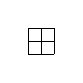
\begin{tikzpicture}[scale=1, transform shape]
			\draw[step={0.5/3}] (0,0) grid ++(1/3,1/3);
		\end{tikzpicture}
	}(x)
	=
	1+4x+2x^2
\]

\[
	P_
	{
		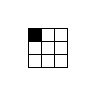
\begin{tikzpicture}[scale=1, transform shape]
			\draw[step={0.5/3}] (0,0) grid ++(0.5,0.5);
			\filldraw (0,1/3) rectangle ++(0.5/3,0.5/3);
		\end{tikzpicture}
	}
	(x)
	=xP_
	{
		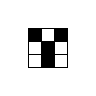
\begin{tikzpicture}[scale=1, transform shape]
			\draw[step={0.5/3}] (0,0) grid ++(0.5,0.5);
			\filldraw (0,1/3) rectangle ++(0.5/3,0.5/3);
			\filldraw (1/3,1/3) rectangle ++(0.5/3,0.5/3);
			\filldraw (0.5/3,0.5/3) rectangle ++(0.5/3,0.5/3);
			\filldraw (0.5/3,0) rectangle ++(0.5/3,0.5/3);
		\end{tikzpicture}
	}(x)
	+P_
	{
		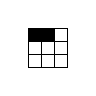
\begin{tikzpicture}[scale=1, transform shape]
			\draw[step={0.5/3}] (0,0) grid ++(0.5,0.5);
			\filldraw (0,1/3) rectangle ++(0.5/3,0.5/3);
			\filldraw (0.5/3,1/3) rectangle ++(0.5/3,0.5/3);
		\end{tikzpicture}
	}(x)
\]
\[
	xP_
	{
		
\begin{tikzpicture}[scale=1, transform shape]
			\draw[step={0.5/3}] (0,0) grid ++(0.5,0.5);
			\filldraw (0,1/3) rectangle ++(0.5/3,0.5/3);
			\filldraw (0.5/3,1/3) rectangle ++(0.5/3,0.5/3);
			\filldraw (1/3,1/3) rectangle ++(0.5/3,0.5/3);
			\filldraw (0.5/3,0.5/3) rectangle ++(0.5/3,0.5/3);
			\filldraw (0.5/3,0) rectangle ++(0.5/3,0.5/3);
		\end{tikzpicture}
	}(x)
	=
	P_
	{
		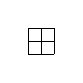
\begin{tikzpicture}[scale=1, transform shape]
			\draw[step={0.5/3}] (0,0) grid ++(1/3,1/3);
		\end{tikzpicture}
	}(x)
	=1+4x+2x^2
\]
\[
	P_
	{
		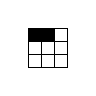
\begin{tikzpicture}[scale=1, transform shape]
			\draw[step={0.5/3}] (0,0) grid ++(0.5,0.5);
			\filldraw (0,1/3) rectangle ++(0.5/3,0.5/3);
			\filldraw (0.5/3,1/3) rectangle ++(0.5/3,0.5/3);
		\end{tikzpicture}
	}(x)
	=xP_
	{
		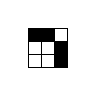
\begin{tikzpicture}[scale=1, transform shape]
			\draw[step={0.5/3}] (0,0) grid ++(0.5,0.5);
			\filldraw (0,1/3) rectangle ++(0.5/3,0.5/3);
			\filldraw (0.5/3,1/3) rectangle ++(0.5/3,0.5/3);
			\filldraw (1/3,0.5/3) rectangle ++(0.5/3,0.5/3);
			\filldraw (1/3,0) rectangle ++(0.5/3,0.5/3);
		\end{tikzpicture}
	}(x)+
	P_
	{
		
\begin{tikzpicture}[scale=1, transform shape]
			\draw[step={0.5/3}] (0,0) grid ++(0.5,0.5);
			\filldraw (0,1/3) rectangle ++(0.5/3,0.5/3);
			\filldraw (0.5/3,1/3) rectangle ++(0.5/3,0.5/3);
			\filldraw (1/3,1/3) rectangle ++(0.5/3,0.5/3);
		\end{tikzpicture}
	}(x)
\]
\[
	P_
	{
		
\begin{tikzpicture}[scale=1, transform shape]
			\draw[step={0.5/3}] (0,0) grid ++(0.5,0.5);
			\filldraw (0,1/3) rectangle ++(0.5/3,0.5/3);
			\filldraw (0.5/3,1/3) rectangle ++(0.5/3,0.5/3);
			\filldraw (1/3,1/3) rectangle ++(0.5/3,0.5/3);
		\end{tikzpicture}
	}(x)
	=xP_
	{
		
\begin{tikzpicture}[scale=1, transform shape]
			\draw[step={0.5/3}] (0,0) grid ++(0.5,0.5);
			\filldraw (0,1/3) rectangle ++(0.5/3,0.5/3);
			\filldraw (0.5/3,1/3) rectangle ++(0.5/3,0.5/3);
			\filldraw (1/3,1/3) rectangle ++(0.5/3,0.5/3);

			\filldraw (0.5/3,0.5/3) rectangle ++(0.5/3,0.5/3);
			\filldraw (1/3,0.5/3) rectangle ++(0.5/3,0.5/3);

			\filldraw (0,0) rectangle ++(0.5/3,0.5/3);
		\end{tikzpicture}
	}(x)+
	P_
	{
		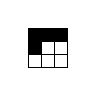
\begin{tikzpicture}[scale=1, transform shape]
			\draw[step={0.5/3}] (0,0) grid ++(0.5,0.5);
			\filldraw (0,0.5/3) rectangle ++(0.5/3,0.5/3);

			\filldraw (0,1/3) rectangle ++(0.5/3,0.5/3);
			\filldraw (0.5/3,1/3) rectangle ++(0.5/3,0.5/3);
			\filldraw (1/3,1/3) rectangle ++(0.5/3,0.5/3);
		\end{tikzpicture}
	}(x)
\]
\[
	P_
	{
		
\begin{tikzpicture}[scale=1, transform shape]
			\draw[step={0.5/3}] (0,0) grid ++(0.5,0.5);
			% y = 0
			\filldraw (0,0) rectangle ++(0.5/3,0.5/3);
			%\filldraw (0.5/3,0) rectangle ++(0.5/3,0.5/3);
			%\filldraw (1/3,0) rectangle ++(0.5/3,0.5/3);

			% y = 1
			\filldraw (0,0.5/3) rectangle ++(0.5/3,0.5/3);
			\filldraw (0.5/3,0.5/3) rectangle ++(0.5/3,0.5/3);
			\filldraw (1/3,0.5/3) rectangle ++(0.5/3,0.5/3);

			% y = 2
			\filldraw (0,1/3) rectangle ++(0.5/3,0.5/3);
			\filldraw (0.5/3,1/3) rectangle ++(0.5/3,0.5/3);
			\filldraw (1/3,1/3) rectangle ++(0.5/3,0.5/3);
		\end{tikzpicture}
	}(x)+
	P_
	{
		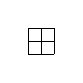
\begin{tikzpicture}[scale=1, transform shape]
			\draw[step={0.5/3}] (0,0) grid ++(1/3,1/3);
		\end{tikzpicture}
	}(x)
	=
	+1+2x
\]
\[
	P_
	{
		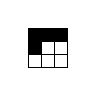
\begin{tikzpicture}[scale=1, transform shape]
			\draw[step={0.5/3}] (0,0) grid ++(0.5,0.5);
			% y = 0
			%\filldraw (0,0) rectangle ++(0.5/3,0.5/3);
			%\filldraw (0.5/3,0) rectangle ++(0.5/3,0.5/3);
			%\filldraw (1/3,0) rectangle ++(0.5/3,0.5/3);

			% y = 1
			\filldraw (0,0.5/3) rectangle ++(0.5/3,0.5/3);
			%\filldraw (0.5/3,0.5/3) rectangle ++(0.5/3,0.5/3);
			%\filldraw (1/3,0.5/3) rectangle ++(0.5/3,0.5/3);

			% y = 2
			\filldraw (0,1/3) rectangle ++(0.5/3,0.5/3);
			\filldraw (0.5/3,1/3) rectangle ++(0.5/3,0.5/3);
			\filldraw (1/3,1/3) rectangle ++(0.5/3,0.5/3);
		\end{tikzpicture}
	}(x)
	=xP_
	{
		
\begin{tikzpicture}[scale=1, transform shape]
			\draw[step={0.5/3}] (0,0) grid ++(0.5,0.5);
			% y = 0
			%\filldraw (0,0) rectangle ++(0.5/3,0.5/3);
			\filldraw (0.5/3,0) rectangle ++(0.5/3,0.5/3);
			\filldraw (1/3,0) rectangle ++(0.5/3,0.5/3);

			% y = 1
			\filldraw (0,0.5/3) rectangle ++(0.5/3,0.5/3);
			%\filldraw (0.5/3,0.5/3) rectangle ++(0.5/3,0.5/3);
			%\filldraw (1/3,0.5/3) rectangle ++(0.5/3,0.5/3);

			% y = 2
			\filldraw (0,1/3) rectangle ++(0.5/3,0.5/3);
			\filldraw (0.5/3,1/3) rectangle ++(0.5/3,0.5/3);
			\filldraw (1/3,1/3) rectangle ++(0.5/3,0.5/3);
		\end{tikzpicture}
	}(x)+
	P_
	{
		
\begin{tikzpicture}[scale=1, transform shape]
			\draw[step={0.5/3}] (0,0) grid ++(0.5,0.5);
			% y = 0
			\filldraw (0,0) rectangle ++(0.5/3,0.5/3);
			%\filldraw (0.5/3,0) rectangle ++(0.5/3,0.5/3);
			%\filldraw (1/3,0) rectangle ++(0.5/3,0.5/3);

			% y = 1
			\filldraw (0,0.5/3) rectangle ++(0.5/3,0.5/3);
			%\filldraw (0.5/3,0.5/3) rectangle ++(0.5/3,0.5/3);
			%\filldraw (1/3,0.5/3) rectangle ++(0.5/3,0.5/3);

			% y = 2
			\filldraw (0,1/3) rectangle ++(0.5/3,0.5/3);
			\filldraw (0.5/3,1/3) rectangle ++(0.5/3,0.5/3);
			\filldraw (1/3,1/3) rectangle ++(0.5/3,0.5/3);
		\end{tikzpicture}
	}(x)
\]

\begin{align*}
	P_
	{
		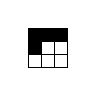
\begin{tikzpicture}[scale=1, transform shape]
			\draw[step={0.5/3}] (0,0) grid ++(0.5,0.5);
			% y = 0
			%\filldraw (0,0) rectangle ++(0.5/3,0.5/3);
			%\filldraw (0.5/3,0) rectangle ++(0.5/3,0.5/3);
			%\filldraw (1/3,0) rectangle ++(0.5/3,0.5/3);
			%
			% y = 1
			\filldraw (0,0.5/3) rectangle ++(0.5/3,0.5/3);
			%\filldraw (0.5/3,0.5/3) rectangle ++(0.5/3,0.5/3);
			%\filldraw (1/3,0.5/3) rectangle ++(0.5/3,0.5/3);
			%
			% y = 2
			\filldraw (0,1/3) rectangle ++(0.5/3,0.5/3);
			\filldraw (0.5/3,1/3) rectangle ++(0.5/3,0.5/3);
			\filldraw (1/3,1/3) rectangle ++(0.5/3,0.5/3);
		\end{tikzpicture}
	}(x)
	&= x(1+2x)+1+4x+2x^2\\
	&= x+2x^2+1+4x+2x^2\\
	&= 1+5x+4x^2
\end{align*}

\begin{align*}
	P_
	{
		
\begin{tikzpicture}[scale=1, transform shape]
			\draw[step={0.5/3}] (0,0) grid ++(0.5,0.5);
			% y = 0
			%\filldraw (0,0) rectangle ++(0.5/3,0.5/3);
			%\filldraw (0.5/3,0) rectangle ++(0.5/3,0.5/3);
			%\filldraw (1/3,0) rectangle ++(0.5/3,0.5/3);
			%
			% y = 1
			%\filldraw (0,0.5/3) rectangle ++(0.5/3,0.5/3);
			%\filldraw (0.5/3,0.5/3) rectangle ++(0.5/3,0.5/3);
			%\filldraw (1/3,0.5/3) rectangle ++(0.5/3,0.5/3);
			%
			% y = 2
			\filldraw (0,1/3) rectangle ++(0.5/3,0.5/3);
			\filldraw (0.5/3,1/3) rectangle ++(0.5/3,0.5/3);
			\filldraw (1/3,1/3) rectangle ++(0.5/3,0.5/3);
		\end{tikzpicture}
	}(x)
	&= x(1+2x)+1+5x+4x^2\\
	&= x+2x^2+1+5x+4x^2\\
	&= 1+6x+6x^2
\end{align*}
\begin{align*}
	P_
	{
		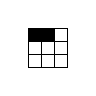
\begin{tikzpicture}[scale=1, transform shape]
			\draw[step={0.5/3}] (0,0) grid ++(0.5,0.5);
			% y = 0
			%\filldraw (0,0) rectangle ++(0.5/3,0.5/3);
			%\filldraw (0.5/3,0) rectangle ++(0.5/3,0.5/3);
			%\filldraw (1/3,0) rectangle ++(0.5/3,0.5/3);
			%
			% y = 1
			%\filldraw (0,0.5/3) rectangle ++(0.5/3,0.5/3);
			%\filldraw (0.5/3,0.5/3) rectangle ++(0.5/3,0.5/3);
			%\filldraw (1/3,0.5/3) rectangle ++(0.5/3,0.5/3);
			%
			% y = 2
			\filldraw (0,1/3) rectangle ++(0.5/3,0.5/3);
			\filldraw (0.5/3,1/3) rectangle ++(0.5/3,0.5/3);
			%\filldraw (1/3,1/3) rectangle ++(0.5/3,0.5/3);
		\end{tikzpicture}
	}(x)
	&= x(1+4x+2x^2) +1+6x+6x^2\\
	&= x+4x^2+2x^3+1+6x+6x^2\\
	&= 1+7x+10x^2+2x^3
\end{align*}
\begin{align*}
	P_
	{
		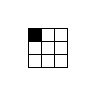
\begin{tikzpicture}[scale=1, transform shape]
			\draw[step={0.5/3}] (0,0) grid ++(0.5,0.5);
			% y = 0
			%\filldraw (0,0) rectangle ++(0.5/3,0.5/3);
			%\filldraw (0.5/3,0) rectangle ++(0.5/3,0.5/3);
			%\filldraw (1/3,0) rectangle ++(0.5/3,0.5/3);
			%
			% y = 1
			%\filldraw (0,0.5/3) rectangle ++(0.5/3,0.5/3);
			%\filldraw (0.5/3,0.5/3) rectangle ++(0.5/3,0.5/3);
			%\filldraw (1/3,0.5/3) rectangle ++(0.5/3,0.5/3);
			%
			% y = 2
			\filldraw (0,1/3) rectangle ++(0.5/3,0.5/3);
			%\filldraw (0.5/3,1/3) rectangle ++(0.5/3,0.5/3);
			%\filldraw (1/3,1/3) rectangle ++(0.5/3,0.5/3);
		\end{tikzpicture}
	}(x)
	&= x(1+4x+2x^2)+1+7x+10x^2+2x^3\\
	&= x+4x^2+2x^3+1+7x+10x^22x^3\\
	&= 1+8x+14x^2+4x^3
\end{align*}
\begin{align*}
	P_
	{
		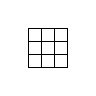
\begin{tikzpicture}[scale=1, transform shape]
			\draw[step={0.5/3}] (0,0) grid ++(0.5,0.5);
			% y = 0
			%\filldraw (0,0) rectangle ++(0.5/3,0.5/3);
			%\filldraw (0.5/3,0) rectangle ++(0.5/3,0.5/3);
			%\filldraw (1/3,0) rectangle ++(0.5/3,0.5/3);
			%
			% y = 1
			%\filldraw (0,0.5/3) rectangle ++(0.5/3,0.5/3);
			%\filldraw (0.5/3,0.5/3) rectangle ++(0.5/3,0.5/3);
			%\filldraw (1/3,0.5/3) rectangle ++(0.5/3,0.5/3);
			%
			% y = 2
			%\filldraw (0,1/3) rectangle ++(0.5/3,0.5/3);
			%\filldraw (0.5/3,1/3) rectangle ++(0.5/3,0.5/3);
			%\filldraw (1/3,1/3) rectangle ++(0.5/3,0.5/3);
		\end{tikzpicture}
	}(x)
	&= x(1+4x+2x^2)+1+8x+14x^2+4x^3\\
	&= x+4x^2+2x^3+1+8x+14x^2+4x^3\\
	&= 1+9x+18x^2+6x^3
\end{align*}

\section{Tablas}%
\label{sec:tablas}
\[
	\begin{cases}
		S_n = 2S_{n-1}+8S_{n-2}\\
		S_0 = 1\\
		S_1 = 2
	\end{cases}
\]

\begin{align*}
	S_nx^n&=2S_{n-1}x^n+8S_{n-2}x^n\\
	\sum_{n=2}^\infty
	S_nx^n &=
	\sum_{n=2}^\infty
	\left(
		2S_{n-1}x^n+8S_{n-2}x^n
	\right)\\
	\\
	S(x) &=
	\sum_{n=2}^\infty
	S_nx^n\\
	\\
	S(x)-S_1x^1-S_0&=
	\sum_{n=2}^\infty
	2S_{n-1}x^n
	+
	\sum_{n=2}^\infty
	8S_{n-2}x^n\\
	S(x)-S_1x^1-S_0&=
	2x
	\sum_{n=2}^\infty
	\underbrace
	{
		S_{n-1}x^{n-1}
	}_
	{
		S(x)-S_0
	}
	+
	8x^2
	\sum_{n=2}^\infty
	\underbrace
	{
		S_{n-2}x^{n-2}
	}_
	{
		S(x)
	}\\
	S(x)-2x+1 &=
	2x(S(x)-1)+8x^2S(x)\\
	\cancel{-2x}
	-1
	\cancel{2x} &=
	S(x)(8x^2+2x-1)\\
	\frac{-1}{8x^2+2x-1} &= S(x)
\end{align*}

\begin{align*}
	S(x) &= \frac{-1}{8x^2+2x-1} \\
	S(x) &= \frac{-1}{(4x-1)(2x+1)} \\
	\\
	\frac{-1}{(4x-1)(2x+1)} &=
	\frac{A}{4x-1} + \frac{B}{2x+1} \\
	-1 &= A(2x+1) + B(4x-1)
	\intertext{$x=-0.5$:}
	-1 &= \cancel{ A(-1+1) } + B(-2-1)\\
	-1 &= -3B\\
	B &= \frac{1}{3}
	\intertext{$x=0.25$:}
	-1 &= A(0.5+1)+ \cancel{B(1-1)}\\
	-1 &= 1.5A\\
	A &= \frac{-2}{3} \\
	\\
	S(x) &= \frac{ - \frac{2}{3} }{4x-1}
	+
	\frac{ \frac{1}{3} }{2x+1}\\
	S(x) &= \frac{2}{3} * \frac{1}{1-4x}
	+
	\frac{1}{3} * \frac{1}{1-(-2x)}\\
	S(x) &= \frac{2}{3} *
	\sum_{k=0}^\infty
	4^kx^k
	+
	\frac{1}{3} *
	\sum_{k=0}^\infty
	(-2)^kx^k\\
	S(x) &=
	\sum_{k=0}^\infty
	\left(
		\frac{2}{3} 4^k
		+
		\frac{1}{3} (-2)^k
	\right)x^k\
	\\
	S_k &= \frac{2}{3} 4^k + \frac{1}{3} (-2)^k
\end{align*}

\end{document}
%}}}
